\section{Fresnel with complex index}

The second example extends the single-interface benchmark to a complex
refractive index and adds the phase of the reflected amplitude as an
independent check. Two cases are evaluated side by side at
$\lambda = \SI{550}{\nano\metre}$: air ($n_0 = 1.00$) against a
non-absorbing glass substrate ($n_1 = 1.50$), and air against an absorbing
Si-like substrate ($n_1 = 4.00 + 0.05\,\ii$). The angle of incidence is
sampled from $0$ to \SI{89.5}{\degree} in 361 points. Because the substrate
can be complex, Snell's law and the cosine that enters
\eqref{eq:fresnel-rs}--\eqref{eq:fresnel-rp} must be evaluated on the
physical branch,
\begin{equation}
  \cos\theta_1 = \sqrt{1 - (n_0/n_1)^{2}\sin^{2}\theta_0},\qquad \Imy(\cos\theta_1)\ge 0, \label{eq:cos-branch}
\end{equation}
so that the transmitted wave decays into the absorbing half-space. At
normal incidence the two polarisations become physically indistinguishable
and the code returns
\begin{equation}
  r_s(0) = r_p(0) = \frac{n_0 - n_1}{n_0 + n_1}, \label{eq:fresnel2-normal}
\end{equation}
whereas the textbook formulas written in the opposite sign convention give
$r_s(0) = -r_p(0)$; the sign flip is applied once when overlaying the
analytic reference on the TMM curve.

\begin{center}
\begin{tikzpicture}
  \fill[black!4] (0,0) rectangle (5,1.8);
  \fill[red!6]   (0,-1.2) rectangle (5,0);
  \draw[thick] (0,0) -- (5,0);
  \node[lbl, anchor=east] at (4.9, 1.4) {$n_0=1$};
  \node[lbl, anchor=east] at (4.9,-0.8) {$n_1 \in \mathbb{C}$};
  \raysketch{1.6}{35}{f}
\end{tikzpicture}
\end{center}

\begin{figure}[!htbp]
  \centering
  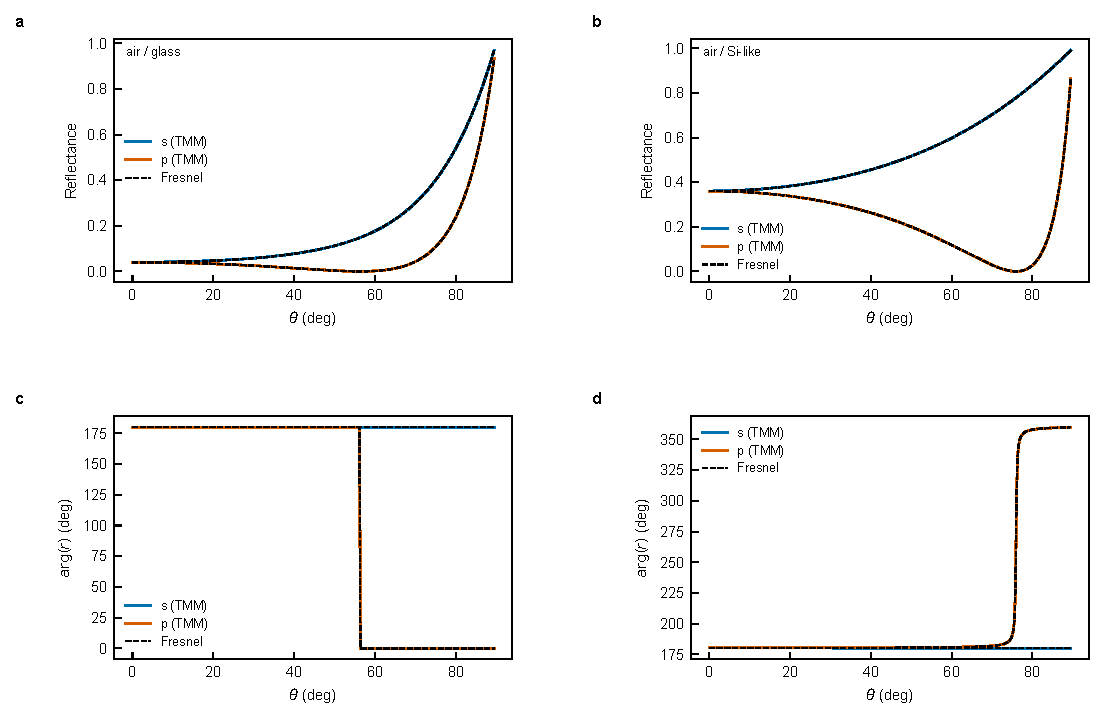
\includegraphics[width=\textwidth]{02_fresnel_analytic_check.pdf}
  \caption{TMM versus closed-form Fresnel for a real (glass) and a complex (Si-like) substrate. Panels (a,b) show $R_s(\theta)$ and $R_p(\theta)$; panels (c,d) show $\arg r_s$ and $\arg r_p$ over the same angular range.}
  \label{fig:fresnel2}
\end{figure}

With the sign convention fixed, amplitudes and phases coincide in all
four panels at $\max|\Delta R| \approx \num{6e-14}$. The dielectric case
shows the expected sharp Brewster zero and $\pi$ phase jump in $r_p$, while
the absorbing substrate replaces both by the smooth phase walk of
Fig.~\ref{fig:fresnel2}(d). The agreement across real and complex
substrates validates the branch-cut choice of~\eqref{eq:cos-branch}, which
is the single numerical subtlety that separates the complex case from the
real one.


